\documentclass[12pt,tikz,border=10pt]{standalone}
\usetikzlibrary{arrows.meta, positioning, calc, decorations.pathreplacing}
\usepackage{amsmath}
\usepackage{amssymb}

\begin{document}
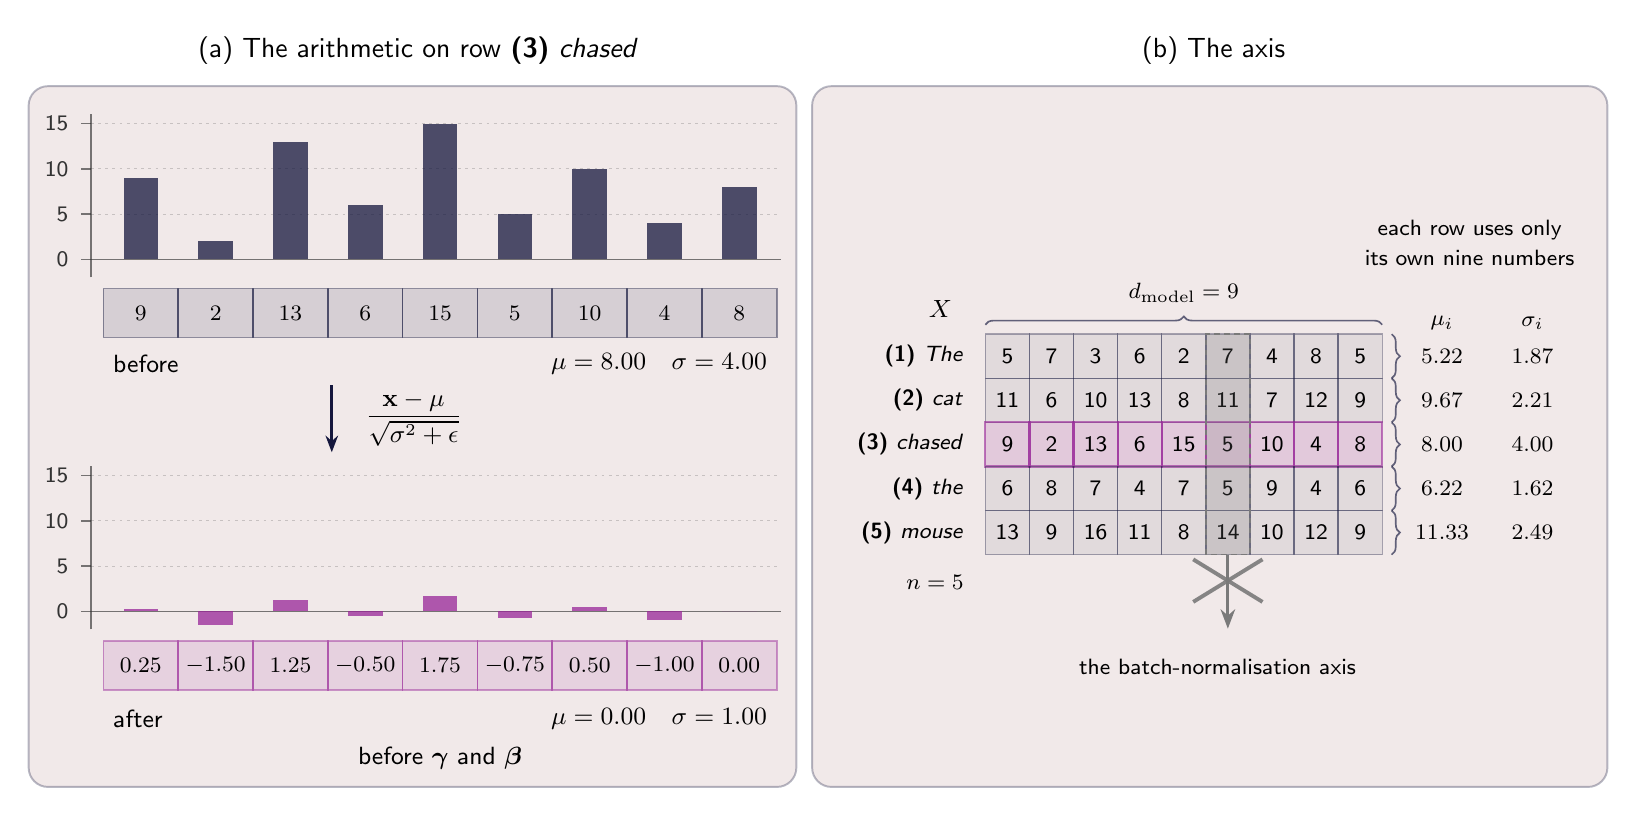
\begin{tikzpicture}[
    every node/.style={font=\sffamily},
]

\definecolor{c1}{HTML}{15173D}
\definecolor{c2}{HTML}{982598}
\definecolor{c3}{HTML}{E491C9}
\definecolor{c4}{HTML}{F1E9E9}
\definecolor{axiscolor}{HTML}{333333}
\definecolor{labelcolor}{HTML}{000000}
\definecolor{bnorm}{HTML}{7A7A7A}

% ================================================================
%  THE ARITHMETIC, computed and not invented.  Audit it here.
%
%  Row (3) chased of X, d_model = 9, in the order drawn:
%      x = [ 9, 2, 13, 6, 15, 5, 10, 4, 8 ]
%  sum = 9+2+13+6+15+5+10+4+8 = 72
%  mu  = 72 / 9 = 8.0000                                -> 8.00
%  deviations x - mu:
%      [ 1, -6, 5, -2, 7, -3, 2, -4, 0 ]     (they sum to 0)
%  squares:
%      [ 1, 36, 25, 4, 49, 9, 4, 16, 0 ]     sum = 144
%  sigma^2 = 144 / 9 = 16.0000 ; sigma = 4.0000          -> 4.00
%  eps = 1e-5, so sqrt(sigma^2 + eps) = 4.00000125: it moves nothing
%  at two decimals, and the printed quotients below use /4 exactly.
%  (x - mu) / sqrt(sigma^2 + eps):
%      [ 0.25, -1.50, 1.25, -0.50, 1.75, -0.75, 0.50, -1.00, 0.00 ]
%  those nine sum to 0.00 and have population sd exactly 1.00.
%  gamma and beta are deliberately NOT applied; the figure says so.
%
%  The other four rows of X, each with its own statistics
%  (population variance, 1/d, two decimals):
%   (1) The     [ 5, 7, 3, 6, 2, 7, 4, 8, 5]  sum 47  mu 5.2222  -> 5.22
%                 sum sq dev = 31.5556, /9 = 3.5062, sd 1.8725 -> 1.87
%   (2) cat     [11, 6,10,13, 8,11, 7,12, 9]  sum 87  mu 9.6667  -> 9.67
%                 sum sq dev = 44.0000, /9 = 4.8889, sd 2.2111 -> 2.21
%   (3) chased  [ 9, 2,13, 6,15, 5,10, 4, 8]  sum 72  mu 8.0000  -> 8.00
%                 sum sq dev =144.0000, /9 =16.0000, sd 4.0000 -> 4.00
%   (4) the     [ 6, 8, 7, 4, 7, 5, 9, 4, 6]  sum 56  mu 6.2222  -> 6.22
%                 sum sq dev = 23.5556, /9 = 2.6173, sd 1.6178 -> 1.62
%   (5) mouse   [13, 9,16,11, 8,14,10,12, 9]  sum 102 mu 11.3333 -> 11.33
%                 sum sq dev = 56.0000, /9 = 6.2222, sd 2.4944 -> 2.49
%  Five different pairs.  No sum anywhere crosses a row boundary.
%
%  GEOMETRY, planned before any TikZ was written.
%
%  Two panels sharing one band, y in [-2.15, 6.75], titles at 6.90.
%    (a) rect x [-0.95, 8.95]      (b) rect x [9.35, 18.80]
%
%  PANEL (a), one row twice, stacked, on ONE shared value axis.
%    cells 0.95 x 0.62, nine of them, x from 0 to 8.55,
%      cell c centre x = 0.475 + 0.95c
%    bar strip: u = 0.115 cm per unit, axis from v = -2 to v = 16,
%      so each strip is 2.07 cm tall; bars 0.44 wide on the cell centre
%    BEFORE  zero line y = 4.55, top 6.39, bottom 4.32,
%            grid 5 -> 5.125, 10 -> 5.700, 15 -> 6.275
%            cells 3.56..4.18, caption line y = 3.22
%    arrow   x = 2.90, from 2.95 down to 2.10; the formula sits to its
%            right, anchored west at (3.20, 2.52)
%    AFTER   zero line y = 0.08, top 1.92, bottom -0.15, same grid
%            offsets; cells -0.92..-0.30, caption line y = -1.28
%            note "before gamma and beta" centred (4.275, -1.78)
%    Both strips carry the same four ticks, so the after bars are read
%    against the height the before bars reached.
%
%  PANEL (b), the 5 x 9 matrix.
%    cells 0.56 square, matrix left 11.20, right 16.24,
%      row i top = 4.30 - 0.56(i-1), so rows run 4.30 down to 1.50
%    row labels anchored east at x = 11.05 ; n = 5 stamp at (10.30, 1.15)
%    top brace 11.20..16.24 at y = 4.42, d_model label at 4.58
%    per-row brace at x = 16.36 drawn top -> bottom so it opens right
%    stats columns centred at x = 17.00 (mu) and 18.15 (sigma),
%      headers on the same 4.42 line as the top brace
%    struck column = column 6 (index 5), x 14.00..14.56, centre 14.28:
%      grey wash over the five cells, a grey arrow below it from 1.40
%      to 0.95 and a cross at (14.28, 1.20) striking that arrow
%    annotations: batch axis label centred (14.10, 0.58);
%      "each row uses only / its own nine numbers" at x = 17.55,
%      y = 0.72 and 0.37, directly under the statistics it explains
% ================================================================

\tikzset{
  panel/.style={fill=c4, rounded corners=7pt, draw=c1, draw opacity=0.30,
                line width=0.7pt},
  title/.style={font=\sffamily\normalsize, text=black, anchor=south},
  lab/.style={font=\sffamily\small, text=black},
  note/.style={font=\sffamily\small, text=black},
  cellnum/.style={font=\sffamily\footnotesize, text=black},
  tick/.style={font=\sffamily\footnotesize, text=axiscolor, anchor=east},
  grid/.style={draw=axiscolor, draw opacity=0.22, line width=0.4pt,
               dash pattern=on 1pt off 1.6pt},
  zero/.style={draw=axiscolor, draw opacity=0.65, line width=0.6pt},
  ax/.style={draw=axiscolor, draw opacity=0.65, line width=0.6pt},
  arr/.style={-{Stealth[length=6pt]}, line width=1.1pt, draw=c1},
  brc/.style={decorate, decoration={brace, amplitude=3pt}, draw=c1,
              draw opacity=0.65, line width=0.6pt},
}

\def\cw{0.95}   % panel (a) cell width
\def\ch{0.62}   % panel (a) cell height
\def\uu{0.115}  % cm per unit on the shared value axis
\def\bw{0.44}   % bar width
\def\mw{0.56}   % panel (b) cell size

% ---------------------------------------------------------------- panels
\draw[panel] (-0.95, -2.15) rectangle (8.80, 6.75);
\draw[panel] (9.00, -2.15) rectangle (19.10, 6.75);
\node[title] at (4.00, 6.90) {(a) The arithmetic on row \textbf{(3)} \emph{chased}};
\node[title] at (14.10, 6.90) {(b) The axis};

% ================================================================ panel (a)
% one strip: #1 = zero-line y, #2 = colour, #3 = comma list of values
\newcommand{\barstrip}[3]{%
  % the shared axis: same range, same ticks, in both strips
  \draw[ax] (-0.16, {#1-2*\uu}) -- (-0.16, {#1+16*\uu});
  \foreach \v in {0,5,10,15} {
    \draw[ax] (-0.16, {#1+\v*\uu}) -- (-0.28, {#1+\v*\uu});
    \node[tick] at (-0.32, {#1+\v*\uu}) {\v};
  }
  \foreach \v in {5,10,15} {
    \draw[grid] (-0.16, {#1+\v*\uu}) -- (8.60, {#1+\v*\uu});
  }
  \draw[zero] (-0.16, #1) -- (8.60, #1);
  \foreach \v [count=\c from 0] in {#3} {
    \fill[#2, opacity=0.75]
      ({0.475+\cw*\c-0.5*\bw}, #1) rectangle ++(\bw, {\v*\uu});
  }
}

% one row of nine cells: #1 = bottom y, #2 = colour, #3 = values
\newcommand{\cellrow}[3]{%
  \foreach \v [count=\c from 0] in {#3} {
    \fill[#2, opacity=0.12] ({\cw*\c}, #1) rectangle ++(\cw, \ch);
    \draw[#2, opacity=0.45, line width=0.6pt]
      ({\cw*\c}, #1) rectangle ++(\cw, \ch);
    \node[cellnum] at ({\cw*\c+0.5*\cw}, {#1+0.5*\ch}) {$\v$};
  }
}

% ---- before
\barstrip{4.55}{c1}{9,2,13,6,15,5,10,4,8}
\cellrow{3.56}{c1}{9,2,13,6,15,5,10,4,8}
\node[lab, anchor=west] at (0.00, 3.22) {before};
\node[lab, anchor=east] at (8.55, 3.22) {$\mu = 8.00$\quad$\sigma = 4.00$};

% ---- the step
\draw[arr] (2.90, 2.95) -- (2.90, 2.10);
\node[lab, anchor=west] at (3.20, 2.52)
  {$\dfrac{\mathbf{x} - \mu}{\sqrt{\sigma^{2} + \epsilon}}$};

% ---- after
\barstrip{0.08}{c2}{0.25,-1.50,1.25,-0.50,1.75,-0.75,0.50,-1.00,0.00}
\cellrow{-0.92}{c2}{0.25,-1.50,1.25,-0.50,1.75,-0.75,0.50,-1.00,0.00}
\node[lab, anchor=west] at (0.00, -1.28) {after};
\node[lab, anchor=east] at (8.55, -1.28) {$\mu = 0.00$\quad$\sigma = 1.00$};
\node[note] at (4.275, -1.78) {before $\boldsymbol{\gamma}$ and $\boldsymbol{\beta}$};

% ================================================================ panel (b)
\def\ml{11.20}
\def\rt{3.60}

% ---- cells
\foreach \vals [count=\i from 1] in {%
  {5,7,3,6,2,7,4,8,5},
  {11,6,10,13,8,11,7,12,9},
  {9,2,13,6,15,5,10,4,8},
  {6,8,7,4,7,5,9,4,6},
  {13,9,16,11,8,14,10,12,9}} {
  \pgfmathsetmacro{\yb}{\rt - \i*\mw}
  \foreach \v [count=\c from 0] in \vals {
    \ifnum\i=3
      \fill[c2, opacity=0.16] ({\ml+\mw*\c}, \yb) rectangle ++(\mw, \mw);
      \draw[c2, opacity=0.60, line width=0.8pt]
        ({\ml+\mw*\c}, \yb) rectangle ++(\mw, \mw);
    \else
      \fill[c1, opacity=0.07] ({\ml+\mw*\c}, \yb) rectangle ++(\mw, \mw);
      \draw[c1, opacity=0.35, line width=0.5pt]
        ({\ml+\mw*\c}, \yb) rectangle ++(\mw, \mw);
    \fi
    \node[cellnum] at ({\ml+\mw*\c+0.5*\mw}, {\yb+0.5*\mw}) {\v};
  }
}

% ---- row labels, braces, statistics
\foreach \w/\m/\s [count=\i from 1] in {%
  The/5.22/1.87, cat/9.67/2.21, chased/8.00/4.00,
  the/6.22/1.62, mouse/11.33/2.49} {
  \pgfmathsetmacro{\yc}{\rt - \i*\mw + 0.5*\mw}
  \pgfmathsetmacro{\yt}{\rt - \i*\mw + \mw}
  \pgfmathsetmacro{\yb}{\rt - \i*\mw}
  \node[cellnum, anchor=east] at (11.05, \yc) {\textbf{(\i)} \emph{\w}};
  \draw[brc] (16.36, \yt) -- (16.36, \yb);
  \node[cellnum] at (17.00, \yc) {$\m$};
  \node[cellnum] at (18.15, \yc) {$\s$};
}
\node[cellnum] at (17.00, 3.74) {$\mu_i$};
\node[cellnum] at (18.15, 3.74) {$\sigma_i$};
\node[cellnum, anchor=east] at (11.05, 0.45) {$n = 5$};

% ---- width brace
\draw[brc] (\ml, 3.72) -- (16.24, 3.72);
\node[cellnum, anchor=south] at (13.72, 3.88) {$d_{\mathrm{model}} = 9$};
\node[lab, anchor=east] at (10.90, 3.92) {$X$};

% ---- the column batch normalisation would have taken
\fill[bnorm, opacity=0.22] (14.00, 0.80) rectangle (14.56, 3.60);
\draw[bnorm, line width=0.6pt, dash pattern=on 2pt off 1.6pt]
  (14.00, 0.80) rectangle (14.56, 3.60);
\draw[bnorm, line width=1.1pt, -{Stealth[length=7pt]}] (14.28, 0.80) -- (14.28, -0.14);
\draw[bnorm, opacity=0.9, line width=1.4pt] (13.84, 0.74) -- (14.72, 0.20);
\draw[bnorm, opacity=0.9, line width=1.4pt] (13.84, 0.20) -- (14.72, 0.74);
\node[cellnum] at (14.15, -0.62) {the batch-normalisation axis};

% ---- the point of the panel, set beside the statistics it explains
\node[cellnum] at (17.35, 4.92) {each row uses only};
\node[cellnum] at (17.35, 4.57) {its own nine numbers};

\end{tikzpicture}
\end{document}
